\documentclass[11pt]{article}

\usepackage{amsmath}
\usepackage{amssymb}
\usepackage[letterpaper,margin=0.72in,headheight=15pt]{geometry}
\usepackage{array}
\usepackage{booktabs}
\usepackage{fancyhdr}
\usepackage{graphicx}
\usepackage{listings}
\usepackage{microtype}
\usepackage{tabularx}
\usepackage{tikz}
\usepackage{xcolor}
\usepackage[hidelinks]{hyperref}

\hypersetup
{
    pdftitle={ADK Lesson 008: Calibrate and stabilize a sampled signal},
    pdfauthor={Kevin Shanahan},
    pdfsubject={Deterministic calibration, moving average, and deadband},
    pdflang={en-US}
}

\usetikzlibrary{arrows.meta,positioning}
\graphicspath{{docs/lessons/assets/}{../assets/}}

\definecolor{ink}{HTML}{20252A}
\definecolor{soft}{HTML}{F3F2EE}
\definecolor{mid}{HTML}{6F777B}
\definecolor{accent}{HTML}{3E5964}
\definecolor{codebg}{HTML}{F7F7F4}

\pagestyle{fancy}
\fancyhf{}
\lhead{\textsc{ADK field lesson 008}}
\rhead{Stable sampled signals}
\cfoot{\thepage}
\setlength{\parindent}{0pt}
\setlength{\parskip}{5pt}
\renewcommand{\arraystretch}{1.18}

\lstdefinestyle{adkcpp}
{
    language=C++,
    basicstyle=\ttfamily\small,
    backgroundcolor=\color{codebg},
    frame=single,
    rulecolor=\color{mid},
    columns=fullflexible,
    keepspaces=true,
    showstringspaces=false,
    keywordstyle=\bfseries\color{accent},
    commentstyle=\itshape\color{mid},
    breaklines=true,
    tabsize=4
}

\newcommand{\checkbox}{\(\square\)}
\newcommand{\blankline}{\rule{0.96\linewidth}{0.35pt}}

\newenvironment{checkpoint}[1]
{\begin{center}\begin{minipage}{0.94\linewidth}\textbf{Check --- #1}\par}
{\end{minipage}\end{center}}

\begin{document}

\begin{center}
    {\Huge\bfseries Make every transformation visible}\\[3pt]
    {\Large Lesson 008: calibrate and stabilize a sampled signal}\\[7pt]
    \textit{Predict $\rightarrow$ sample $\rightarrow$ map $\rightarrow$
    average $\rightarrow$ hold $\rightarrow$ observe}
\end{center}

\begin{center}
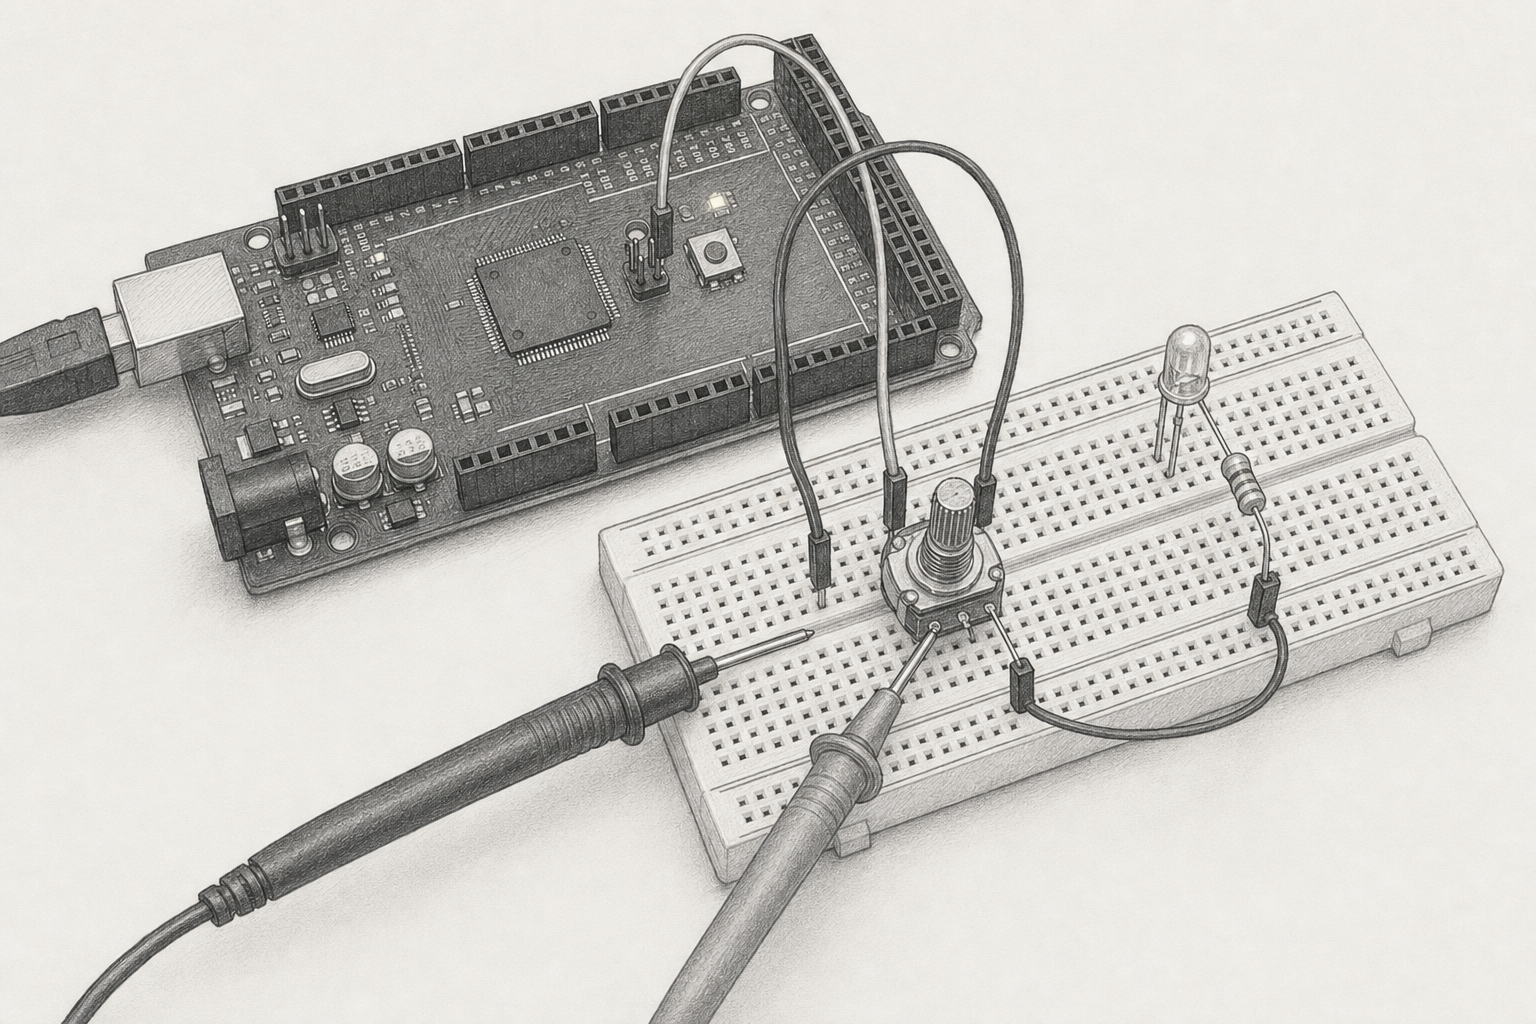
\includegraphics[width=\linewidth,height=0.28\textheight,keepaspectratio]
    {008-sampled-signal-pencil.png}
\end{center}

\textbf{Orientation plate.}
Use the pencil view to identify the three observable places: the knob,
\textbf{TP-A0}, and the brightness LED. It is not a pin map. The exact net list
and schematic below are authoritative.

\begin{tabularx}{\linewidth}{@{}>{\bfseries}lX@{}}
Question & Can explicit, replayable transformations reduce visible jitter
without hiding what the circuit measured?\\
Time & 75--100 minutes\\
Prerequisites & Lesson 007; integer ranges; explicit status handling\\
You need & Mega 2560, USB cable, breadboard, 10\,k\(\Omega\) linear
potentiometer, LED, resistor of at least 220\,\(\Omega\), jumpers, multimeter\\
Evidence & TP-A0 voltage, raw and transformed worksheet, D6 duty/brightness,
D13 acquisition witness, safe-state record\\
Safety class & E1: USB-powered Mega and passive low-current parts only\\
Status & Host-verified and experimental; physical acceptance remains open\\
\end{tabularx}

\section*{Safety boundary}

Remove USB before wiring or moving a probe connection. Use a 10\,k\(\Omega\)
potentiometer between Mega 5\,V and GND; connect only its wiper to A0. Drive
the external LED from D6 through its own resistor of at least
220\,\(\Omega\). All grounds are common.

Filtering is interpretation, not electrical protection. It cannot make an
over-voltage safe, prove a wire is sound, or turn a floating input into valid
evidence. A rail endpoint can be a real knob position or a fault. A disconnected
A0 can wander through plausible values.

\textbf{Stop} for heat, odor, smoke, USB disconnects, a voltage outside
0--5\,V, an unidentified potentiometer terminal, or an unknown resistor.
Disconnect USB upstream; do not move powered breadboard wiring.

\begin{checkpoint}{before wiring}
\checkbox\ USB removed \quad \checkbox\ pot resistance and terminals identified
\quad \checkbox\ LED resistor measured \quad \checkbox\ common ground traced
\end{checkpoint}

\section*{1. Reuse a controlled source}

A controlled potentiometer is deliberately retained from Lesson 007. It lets
you hold, step, and repeat the input before Lesson 009 adds a photoresistor's
environmental variability.

\begin{center}
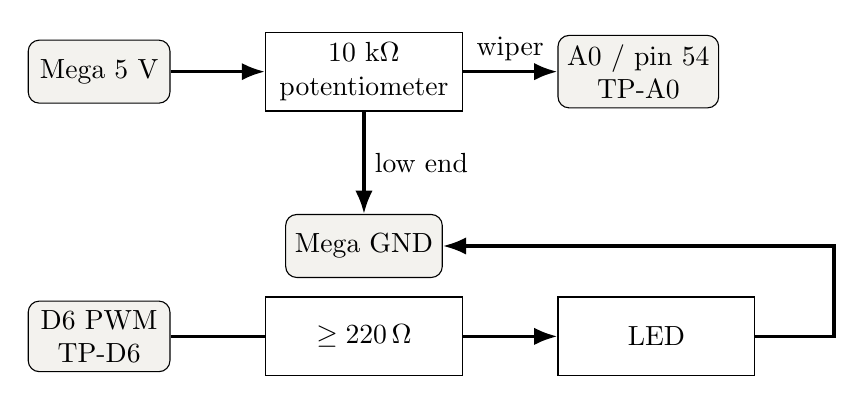
\begin{tikzpicture}[>=Latex,node distance=12mm,
    terminal/.style={draw,rounded corners,fill=soft,minimum width=18mm,
                     minimum height=8mm,align=center},
    part/.style={draw,minimum width=25mm,minimum height=10mm,align=center}]
    \node[terminal] (vcc) {Mega 5 V};
    \node[part,right=of vcc] (pot) {10 k\(\Omega\)\\potentiometer};
    \node[terminal,right=of pot] (a0) {A0 / pin 54\\TP-A0};
    \node[terminal,below=13mm of pot] (gnd) {Mega GND};
    \draw[very thick,->] (vcc)--(pot);
    \draw[very thick,->] (pot)--node[above]{wiper}(a0);
    \draw[very thick,->] (pot)--node[right]{low end}(gnd);

    \node[terminal,below=25mm of vcc] (d6) {D6 PWM\\TP-D6};
    \node[part,right=of d6] (res) {\(\geq220\,\Omega\)};
    \node[part,right=of res] (led) {LED};
    \draw[very thick,->] (d6)--(res)--(led);
    \draw[very thick,->] (led.east)--++(10mm,0)|-(gnd.east);
\end{tikzpicture}
\end{center}

\begin{center}
\begin{tabularx}{0.92\linewidth}{@{}lllX@{}}
\toprule
From & Through & To & Purpose\\
\midrule
Mega 5 V & pot high terminal & --- & known source\\
pot wiper & TP-A0 & Mega A0 & sampled position\\
pot low terminal & --- & Mega GND & divider return\\
Mega D6 & resistor, LED anode & LED cathode to GND & brightness witness\\
Mega D13 & built-in LED & --- & acquisition witness\\
\bottomrule
\end{tabularx}
\end{center}

\section*{2. Predict the evidence chain}

The circuit and program make five different claims. Do not collapse them into
``the LED works.''

\begin{center}
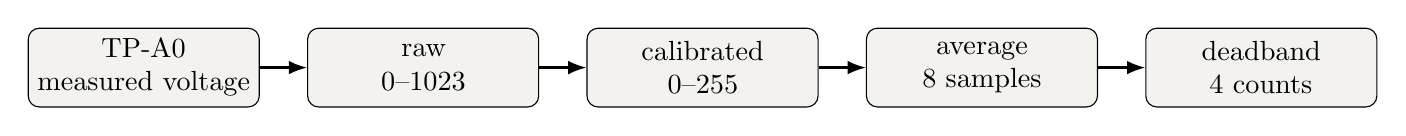
\begin{tikzpicture}[>=Latex,node distance=6mm,
    box/.style={draw,rounded corners,fill=soft,minimum height=10mm,
                text width=27mm,align=center}]
    \node[box] (voltage) {TP-A0\\measured voltage};
    \node[box,right=of voltage] (raw) {raw\\0--1023};
    \node[box,right=of raw] (map) {calibrated\\0--255};
    \node[box,right=of map] (mean) {average\\8 samples};
    \node[box,right=of mean] (hold) {deadband\\4 counts};
    \draw[->,thick] (voltage)--(raw);
    \draw[->,thick] (raw)--(map);
    \draw[->,thick] (map)--(mean);
    \draw[->,thick] (mean)--(hold);
\end{tikzpicture}
\end{center}

D13 on supports the separate claim that all three hardware owners initialized.
D6 brightness and its PWM waveform expose the final held value. TP-A0 remains
available to challenge every software interpretation.

\textbf{Predict.} Before power, write what should happen after a quick knob
step and what should happen while the knob is held still:

\blankline\\[5pt]\blankline

\section*{3. Calibrate observations, not ideal endpoints}

The canonical example maps observed readings 80 through 940 onto duty 0 through
255 and clamps values beyond those observations. These numbers are a repeatable
exercise, not universal facts about your potentiometer.

For an increasing calibration,
\[
y=y_{\min}+
\frac{(x-x_{\min})(y_{\max}-y_{\min})}{x_{\max}-x_{\min}},
\]
with integer rounding. \texttt{LinearCalibration} validates the interval and
returns \texttt{Result<uint16\_t>} because an invalid configuration has no
meaningful mapped result.

\begin{lstlisting}[style=adkcpp]
const adk::LinearCalibrationConfig calibrationConfig{
    80, 940, 0, 255, true};

adk::LinearCalibration calibration (calibrationConfig);

const adk::Result<uint16_t> mapped = calibration.map (raw);
if (!mapped.ok ())
{
    stopSafely ();
}
\end{lstlisting}

\begin{center}
\begin{tabularx}{0.92\linewidth}{@{}lXXXX@{}}
\toprule
Position & TP-A0 & Raw observation & Mapped prediction & Mapped result\\
\midrule
low stop & & & 0 after clamp &\\
quarter & & & &\\
middle & & & &\\
three-quarter & & & &\\
high stop & & & 255 after clamp &\\
\bottomrule
\end{tabularx}
\end{center}

Measure Mega 5\,V and TP-A0 with power on only after placing probes while
unpowered. The ideal relation is
\[
{\rm raw}\approx \frac{V_{\rm TP-A0}}{V_{\rm ref}}\times1023.
\]
Use measured \(V_{\rm ref}\), not an assumed perfect 5.000\,V.

\section*{4. Advance state only from supplied samples}

\texttt{MovingAverage} owns a fixed array of at most 32 readings. The example
uses eight. It has no clock and takes no hidden sample: each
\texttt{addSample()} advances it exactly once. Early results average the
samples received so far.

\texttt{Deadband} publishes the first sample, then retains that value until a
new sample differs by at least its width. It prevents small visible output
changes; it does not erase raw evidence.

\begin{lstlisting}[style=adkcpp]
adk::MovingAverage average        (8);
adk::Deadband      brightnessHold (4);

const adk::Result<uint16_t> smoothed =
    average.addSample (mapped.value ());
const uint16_t stable =
    brightnessHold.addSample (smoothed.value ());
\end{lstlisting}

Order matters. Mapping first gives the deadband a meaning in output duty
counts. Averaging before the deadband lets a real sustained change accumulate.
Reversing these objects would describe a different instrument.

\section*{5. Replay a deterministic sample stream}

Calculate the eight-sample, rounded moving average, then apply a deadband of
four. The initial published value is 100.

\begin{center}
\begin{tabularx}{0.96\linewidth}{@{}rXXXX@{}}
\toprule
Step & Supplied sample & Window contents & Rounded average & Held output\\
\midrule
1 & 100 & 100 & 100 & 100\\
2 & 102 & 100, 102 & &\\
3 & 101 & 100, 102, 101 & &\\
4 & 104 & 100, 102, 101, 104 & &\\
5 & 112 & 100, 102, 101, 104, 112 & &\\
6 & 116 & 100, 102, 101, 104, 112, 116 & &\\
7 & 120 & 100, 102, 101, 104, 112, 116, 120 & &\\
8 & 124 & all eight & &\\
\bottomrule
\end{tabularx}
\end{center}

Replay the same values twice. The result must match at every step. Change only
one sample and identify the first output that can change. This is the central
testability property: the state is a function of configuration and supplied
sample history, not processor speed or wall-clock timing.

\section*{6. Read the narrative run loop}

The canonical sketch introduces owners before transformations. Setup validates
the software configuration, acquires D13, A0, and D6, then lights D13. The loop
reads as observe, decide, actuate:

\begin{lstlisting}[style=adkcpp]
potentiometer.update ();

adk::PwmOutput::Duty brightness = 0;
if (!chooseBrightness (brightness))
{
    stopSafely ();
    return;
}

if (brightnessLed.write (brightness) != adk::Status::Ok)
{
    stopSafely ();
}
\end{lstlisting}

The 20\,ms sampling schedule belongs to the application. Calibration,
averaging, and deadband remain useful in host tests without Arduino time.
Shutdown turns off D6, makes A0 and D6 high impedance, releases all claims, and
turns off D13. Destruction repeats that cleanup safely.

\section*{7. Prove the transforms on the host}

Write deterministic tests before interpreting the breadboard:

\begin{enumerate}
    \item invalid and reversed calibration intervals;
    \item exact endpoints, midpoint rounding, clamping, and unclamped rejection;
    \item moving-average windows 0, 1, 8, 32, and 33;
    \item partial fill, full fill, replacement, reset, and 16-bit extremes;
    \item deadband equality, just inside, just outside, rising, falling, reset;
    \item two identical sample streams with identical result/status traces;
    \item A0 claim conflict and D6 timer conflict before any unintended write;
    \item repeated shutdown and destruction from an active circuit.
\end{enumerate}

\begin{lstlisting}[style=adkcpp]
make host-test
make quality-fast
make arduino-Lesson008SampledSignal
\end{lstlisting}

Compilation and simulation do not establish physical acceptance.

\section*{8. Upload and observe without depending on Serial}

Identify the board and port, compile the one canonical sketch, upload it, and
optionally capture Serial only if a later experiment adds textual records:

\begin{lstlisting}[style=adkcpp]
make boards
make arduino-Lesson008SampledSignal
make upload EXAMPLE=Lesson008SampledSignal PORT=/dev/ttyACM0
make monitor PORT=/dev/ttyACM0 BAUD=115200
\end{lstlisting}

The required evidence is circuit-native:

\begin{enumerate}
    \item D13 off at reset, then steadily on: resource-acquisition witness.
    \item TP-A0 voltage follows the knob: primary input evidence.
    \item D6 duty and LED brightness follow a sustained change: output evidence.
    \item Small TP-A0 movement may leave D6 unchanged: deadband evidence.
    \item A fast step reaches D6 gradually: moving-average evidence.
    \item After the published shutdown procedure, D13 and the LED are off; a
          meter or logic analyzer, not darkness alone, checks safe state.
\end{enumerate}

\begin{center}
\begin{tabularx}{\linewidth}{@{}lXXX@{}}
\toprule
Experiment & Prediction & Observation & Interpretation\\
\midrule
hold at middle & TP-A0 and D6 settle & &\\
small nudge & TP-A0 moves; D6 may hold & &\\
large step & TP-A0 jumps; D6 ramps & &\\
return step & same direction-independent rules & &\\
shutdown & D13/LED off; pins released & &\\
\bottomrule
\end{tabularx}
\end{center}

\section*{9. Diagnose by stage}

\begin{tabularx}{\linewidth}{@{}p{0.22\linewidth}p{0.31\linewidth}X@{}}
\toprule
Observation & Next measurement & What it can establish\\
\midrule
D13 stays off & inspect status path and unpowered wiring & acquisition failed;
not which owner failed without recorded status\\
D13 on, TP-A0 fixed & measure wiper and both pot ends to GND & distinguishes
source wiring from later transforms\\
TP-A0 moves, D6 fixed & inspect expected mapped/average/deadband worksheet;
probe TP-D6 & separates decision from LED wiring\\
D6 waveform changes, LED fixed & remove power; inspect polarity and resistor &
the command reached the pin but the load path is suspect\\
rail reading & inspect all three pot terminals unpowered & may be endpoint or
fault; filtering is not evidence either way\\
plausible wandering input & power off; check A0 continuity & a disconnected
input can float plausibly\\
\bottomrule
\end{tabularx}

\section*{10. Extend the design}

\begin{enumerate}
    \item Reduce the average window from eight to two. Predict response time and
          visible jitter before running it.
    \item Increase the deadband from four to sixteen. Which deliberate knob
          movements disappear?
    \item Swap average and deadband in a host-only experiment. Explain why it
          is a different policy.
    \item Record ten raw endpoint readings, choose observed calibration bounds,
          and justify the margin retained at each end.
    \item Replace the potentiometer samples with a recorded photoresistor trace
          on the host. Do not change hardware yet. Which parameters need
          reconsideration for Lesson 009?
\end{enumerate}

\section*{Bench acceptance record}

\begin{tabularx}{\linewidth}{@{}>{\bfseries}lX@{}}
Board and supply & \\
Meter / analyzer & \\
Measured 5 V reference & \\
Measured pot and LED resistor & \\
Observed calibration bounds & \\
D13 acquisition observation & \\
TP-A0 observations & \\
TP-D6 / brightness observations & \\
Shutdown pin evidence & \\
Deviations, reviewer, date & \\
\end{tabularx}

\begin{checkpoint}{exit}
\checkbox\ source circuit checked unpowered \quad
\checkbox\ every transformation predicted \quad
\checkbox\ deterministic replay passed \quad
\checkbox\ non-Serial evidence recorded \quad
\checkbox\ resource and safe-state evidence kept separate
\end{checkpoint}

\vfill
\small
\textbf{Companion material.}
Use the HTML lesson for current API signatures, canonical source links, errata,
and searchable procedures. Use this PDF for predictions, hand calculations,
stage-by-stage diagnosis, and the physical acceptance record. Until that record
is completed by a person at the named bench, this lesson remains host-verified.

\href{https://docs.arduino.cc/hardware/mega-2560/}
{Arduino Mega 2560 documentation}\quad
\href{https://www.microchip.com/en-us/product/ATmega2560}
{Microchip ATmega2560 datasheet}

\end{document}
